\documentclass[25pt, a0paper, portrait]{tikzposter}
\usepackage{amsmath, amssymb}
\usepackage{graphicx}
\usepackage{booktabs}
\usepackage{xcolor}
\usepackage{helvet}
\usepackage{enumitem}

\makeatletter
\setlength{\TP@blockverticalspace}{18mm}
\setlength{\TP@colspace}{18mm}
\makeatother

\renewcommand{\familydefault}{\sfdefault}

% --- 主题与颜色设置 ---
\usetheme{Simple}
\usecolorstyle{Default}

% 去除标题边框的自定义样式
\definetitlestyle{NoFrame}{
	width=\textwidth, linewidth=0pt, innersep=15mm,
	titletotopverticalspace=15mm, titletoblockverticalspace=15mm,
	titlegraphictotitledistance=10mm, titletextscale=1
}{
	\fill[color=titlebgcolor] (\titleposleft,\titleposbottom) rectangle (\titleposright,\titlepostop);
}
\usetitlestyle{NoFrame}

% --- 科技感配色 ---
\definecolor{TechNavy}{HTML}{0A1633}
\definecolor{TechBlue}{HTML}{DCE9FF}
\definecolor{TechCyan}{HTML}{00D1FF}
\definecolor{TechMint}{HTML}{00E6C3}
\definecolor{TechText}{HTML}{182849}
\definecolor{TechPurple}{HTML}{7B61FF}
\definecolor{TechRose}{HTML}{FF4FB3}
\definecolor{TechBg}{HTML}{F2F7FF}
\definecolor{TechCard}{HTML}{EAF1FF}

\colorlet{backgroundcolor}{TechBg}
\colorlet{framecolor}{TechCyan!68!TechPurple}
\colorlet{titlebgcolor}{TechCard!92!white}
\colorlet{titlefgcolor}{TechNavy}
\colorlet{blocktitlebgcolor}{TechCyan!20!TechPurple!8!white}
\colorlet{blocktitlefgcolor}{TechNavy}
\colorlet{blockbodybgcolor}{white}
\colorlet{blockbodyfgcolor}{TechText}
\colorlet{innerblocktitlebgcolor}{TechPurple!18!TechCyan!8!white}
\colorlet{innerblocktitlefgcolor}{TechNavy}
\colorlet{innerblockbodybgcolor}{TechCard!95!white}
\colorlet{innerblockbodyfgcolor}{TechText}

% --- macOS 窗口风格块 ---
\defineblockstyle{MacWindow}{
titlewidthscale=1, bodywidthscale=1, titleleft,
titleoffsetx=0pt, titleoffsety=0pt, bodyoffsetx=0pt, bodyoffsety=10mm,
bodyverticalshift=10mm, roundedcorners=18, linewidth=1.2pt,
titleinnersep=9mm, bodyinnersep=10mm
}{
\ifBlockHasTitle
\draw[rounded corners=\blockroundedcorners, line width=\blocklinewidth,
color=framecolor, fill=blockbodybgcolor]
(blockbody.south west) rectangle (blockbody.north east);
\draw[rounded corners=\blockroundedcorners, line width=\blocklinewidth,
color=framecolor, fill=blocktitlebgcolor]
(blocktitle.south west) rectangle (blocktitle.north east);
\fi
}
\useblockstyle{MacWindow}

% --- 装饰元素（稳定版）---
\renewcommand{\labelitemi}{\textcolor{TechCyan}{\scriptsize$\bullet$}}
\setlist[itemize]{leftmargin=1.2em, itemsep=0.35em, topsep=0.35em}
\setlist[enumerate]{leftmargin=1.2em, itemsep=0.35em, topsep=0.35em}

\newcommand{\techbadge}[1]{%
\fcolorbox{TechCyan}{TechCard}{\textcolor{TechPurple}{\footnotesize\textbf{\hspace{0.35cm}#1\hspace{0.35cm}}}}%
}

\newcommand{\techicon}{%
\raisebox{-0.1em}{\shortstack[c]{%
\textcolor{red!75!black}{\normalsize$\bullet$}\\[-0.1ex]
\textcolor{orange!80!black}{\normalsize$\bullet$}\\[-0.1ex]
\textcolor{green!60!black}{\normalsize$\bullet$}}}%
\hspace{0.28em}%
}

\newcommand{\techpanel}[1]{%
{\setlength{\fboxsep}{10pt}\fcolorbox{TechCyan}{TechCard}{\parbox{0.9\linewidth}{\centering \vspace{1.8cm} \textcolor{TechPurple}{\textit{#1}} \vspace{1.8cm}}}}%
}

\newcommand{\techpanelsmall}[1]{%
{\setlength{\fboxsep}{9pt}\fcolorbox{TechCyan}{TechCard}{\parbox{0.6\linewidth}{\centering \vspace{1.3cm} \textcolor{TechPurple}{\textit{#1}} \vspace{1.3cm}}}}%
}

% --- 标题信息 ---
\title{%
	\raisebox{-0.5\height}{
\includegraphics[height=8cm]{logo.png}}%
	\hspace{2cm}%
	\parbox[c]{0.8\linewidth}{\centering \textbf{\huge MITIGATING HALLUCINATION IN FINANCIAL RETRIEVAL-AUGMENTED GENERATION \\ VIA FINE-GRAINED KNOWLEDGE VERIFICATION}}%
}
\author{\Large Taoye Yin$^{*}$, Xinya Wu$^{*}$, Haoyuan Hu, Kai Deng, Yaxin Fan, Kezun Zhang, Xinhao Chen, Feng Wang}
\institute{Ant Group, Hangzhou, China}

\begin{document}
	
	\maketitle
	
	\begin{columns}
		
		% ==================== 左栏：痛点与方法 ====================
		\column{0.5}
		
		\block{\techicon 1. Motivation}{
			\begin{itemize}
				\item \textbf{The Problem:} Financial RAG systems rely heavily on retrieved documents, but LLMs still generate hallucinations that contradict the retrieved facts (e.g., temporal or numerical inconsistencies).
				\item \textbf{Existing Solutions:} RL methods typically use coarse binary rewards based on human annotations. This incurs high costs and provides unstable optimization signals.
				\item \textbf{Our Solution:} A Reinforcement Learning framework with \textbf{Fine-grained Knowledge Verification (RLFKV)}.
			\end{itemize}

			\vspace{0.5cm}
			\begin{center}
				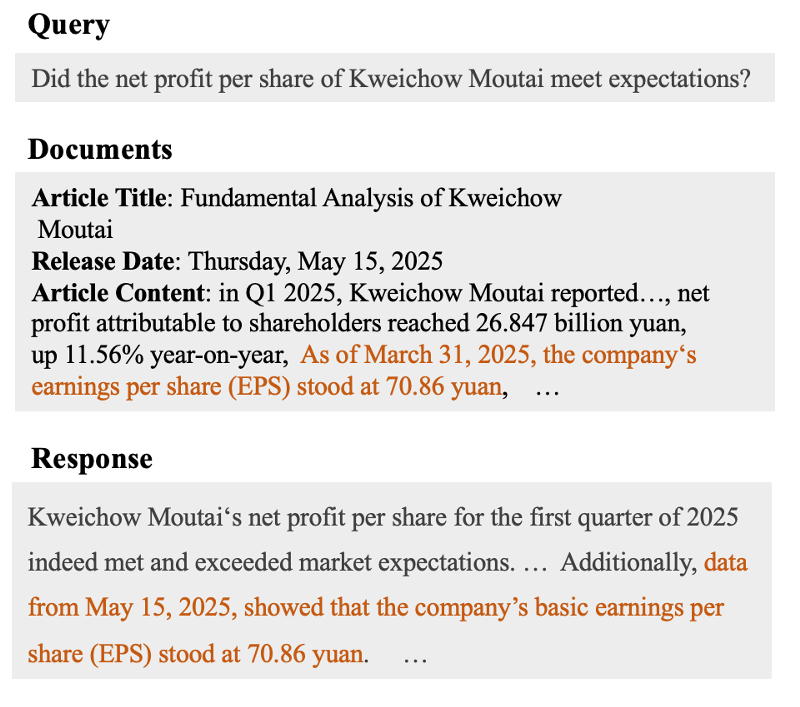
\includegraphics[width=0.7\linewidth]{figure1.png}
			\end{center}
		}
		
		\block{\techicon 2. RLFKV Framework}{
			
			% 建议在这里放置原论文的 Fig. 2 (The framework of RLFKV)
			\begin{center}
				\techpanel{[Insert Fig. 2: RLFKV System Block Diagram Here]}
			\end{center}
			
			\vspace{1cm}
			Our framework optimizes the policy model without manual reference answers through two main steps:
			\begin{enumerate}
				\item \textbf{Decomposition \& Verification:} Decomposes the response into atomic knowledge units (Entity, Metric, Value, Timestamp) and verifies each against retrieved docs.
				\item \textbf{Optimization (GRPO):} Uses verification results to compute fine-grained rewards.
			\end{enumerate}
		}
		
		\block{\techicon 3. Fine-Grained Rewards Formulation}{
			
			We jointly maximize two reward signals to balance faithfulness and prevent reward hacking (overly concise replies).
			
			\vspace{0.5cm}
			\textbf{1. Faithful Reward ($r_f$):} Penalizes factual inconsistencies smoothly.
			\begin{equation}
				r_f = \frac{1}{e^{\eta \cdot \min(\sum_{i=1}^{k} \mathbb{I}(s_i = 0), \gamma)}}
			\end{equation}
			where $s_i \in \{0,1\}$ is the verification score of unit $i$, and $\gamma$ caps the penalty.
			
			\vspace{0.5cm}
			\textbf{2. Informative Reward ($r_i$):} Ensures informational depth matches the base model.
			\begin{equation}
				r_{i}=\begin{cases}1 & \text{if } k \ge k_{0}\\ 0 & \text{otherwise}\end{cases}
			\end{equation}
			where $k_0$ is the number of atomic units generated by the base model $\pi_0$.
		}
		
		% ==================== 右栏：实验与结论 ====================
		\column{0.5}
		
		\block{\techicon 4. Experimental Setup}{
			
			\begin{itemize}
				\item \textbf{Datasets:} Evaluated on BizFinBench \textbf{FDD} (stock-related) and our proposed \textbf{FDD-ANT} (stocks, funds, macroeconomics, 2,000 samples).
				\item \textbf{Baselines:} DeepSeek-V2-Lite, Qwen3-8B, LLaMA3.1-8B, Xuanyuan-13B, Dianjin-R1-7B.
				\item \textbf{Metrics:} Faithfulness (GPT-4o point-wise) and Informativeness (average atomic units).
			\end{itemize}
		}

		\block{\techicon 5. Main Results}{
			
			\textbf{RLFKV effectively reduces hallucination while maintaining informativeness.}
			
			\vspace{1cm}
			% 建议在这里放入原论文的 Table 1 核心数据 或 Fig 3a (柱状图)
			\begin{center}
				\techpanel{[Insert Main Results Table or Fig. 3a Here]}
			\end{center}
			
			\vspace{0.5cm}
			\begin{itemize}
				\item On FDD-ANT, $RLFKV_{Qwen3}$ improves faithfulness by \textbf{3.1 points} over the Qwen3 base model.
				\item Ablation studies show that removing the informative reward drops the informativeness metric significantly, validating its necessity.
			\end{itemize}
		}
		
		\block{\techicon 6. Reward Analysis \& Error Types}{
			
			\textbf{Stability:} Fine-grained rewards demonstrate more stable optimization and converge more rapidly (within 2k steps) compared to coarse-grained binary rewards.
			
			\vspace{0.5cm}
			\textbf{Remaining Challenges:} Error analysis on FDD-ANT reveals three persistent error types:
			\begin{itemize}
				\item \textbf{Time Omission (55\%):} Critical temporal references are absent.
				\item \textbf{Time Error (28\%):} Relative time expressions / calendar year conversions.
				\item \textbf{Numerical Error (17\%):} Imprecise rounding.
			\end{itemize}
			
			% 建议在这里放入 Fig. 4 (饼图)
			\begin{center}
				\techpanelsmall{[Insert Fig. 4 Pie Chart Here]}
			\end{center}
		}
		
		\block{\techicon 7. Conclusion}{
			
			\begin{itemize}
				\item Proposed RLFKV, decomposing responses into verifiable atomic knowledge units.
				\item Achieved consistent improvements in financial RAG factual accuracy without costly human annotations.
				\item Released \textbf{FDD-ANT} dataset to advance real-world financial evaluation.
			\end{itemize}
			
			\vspace{1cm}
			\begin{minipage}{0.7\linewidth}
				\textbf{Scan for Code \& Dataset:} \\
				\textcolor{TechMint}{github.com/antgroup/ANT-Fin-RAG}
			\end{minipage}
			\begin{minipage}{0.25\linewidth}
				% 二维码占位
				\fcolorbox{TechCyan}{TechCard}{\parbox{3cm}{\centering \vspace{1.2cm} \textcolor{TechPurple}{\textbf{QR Code}} \vspace{1.2cm}}}
			\end{minipage}
		}
	\end{columns}
\end{document}